% !TeX root = ../main.tex
% Add the above to each chapter to make compiling the PDF easier in some editors.
\chapter{Methodology}\label{chapter:method}
In order to avoid having a central raw dataset and to eliminate the risk of inference attacks on anonymized data, we propose a framework in which we collect and locally aggregate location data on end user devices (smartphones) through an application designed for this purpose. The raw data will stay on each device and will only be used to serve aggregation requests send from the central server. The aggregation requests have to be defined upfront. An example is the determination of the average number steps per day accross all users. An incoming aggregation request might look like the following:
\begin{lstlisting}[language=json,firstnumber=1]
{
	"start": "2019-05-30",
	"end": "2019-06-02",
	"type": "steps",
	"n" : 3,
	"value": 2000,
	"valueList": []
}
\end{lstlisting}
while the data contained in the outgoing response after processing the request might look like this:
\begin{lstlisting}[language=json,firstnumber=1]
{
	"n" : 4,
	"value": 2500,
	"valueList": []
}
\end{lstlisting}
\begin{figure}[h!]
	\caption{Decentral unencrypted aggregation process}
	\label{decentral-aggregation-unencrypted}
	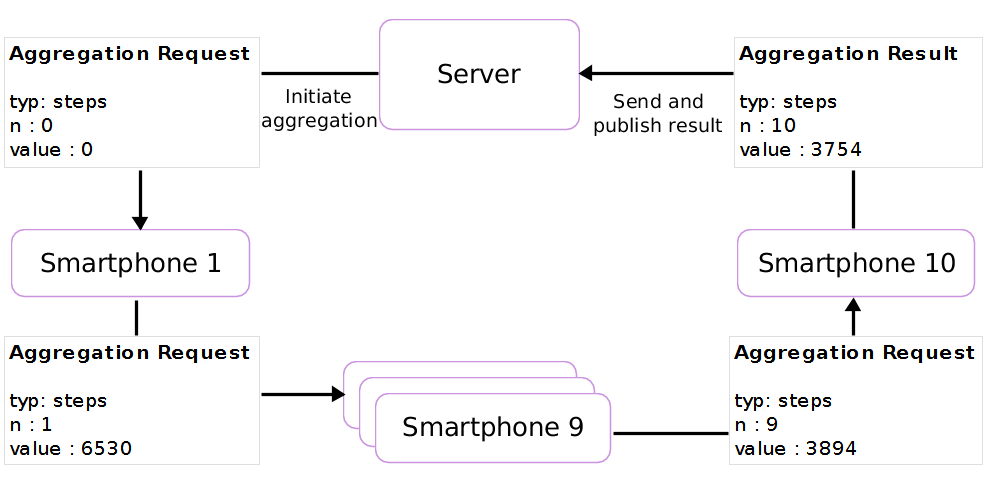
\includegraphics[width=\textwidth]{data/diagrams/decentral-aggregation-6.png}
\end{figure}
Figure \ref{decentral-aggregation-unencrypted} depicts the process of such aggregation request.
 In order to protect the user's privacy and completely shield the raw data from the server, it would be necessary to pass the request via P2P from one device to another until the last device finally sends the results to the server. P2P on mobile phones though is hardly possible. On the other hand, if the server is used to pass an aggreation request from one device to another, it could read the data and compute the respective user's input from the difference. We propose to use encryption in order to hinder the server from reading the data. On installation of the application on a smartphone, a public-private key-pair is generated and every installed application registers at the server with this public key. The corresponding private key is stored locally. On start of an aggregation request, not only the first user but also the following user who should deal with the aggregation request is determmined and the public key of the next user is passed along with the aggregation request. When one end user device needs to send the processed aggregation request to the next phone, it encrypts the data using the provided public key of the next user in the standard hybrid encryption\footnote{In hybrid encryption as used in SSL, the message itself is encrypted with a synchronous key while this key itself is encrypted using the public key} approach leveraging the benefits of synchronous keys. This way the next phone in the aggregation chain will be able to decrypt the request and process the data while the server is unable to read the data until the aggregation request is finally send in plain text for publishing to the server. This process is depicted in figure \ref{decentral-aggregation-encrypted}. This process currently assumes a trusted server and trusted devices. Chapter \ref{chapter:conclusion} discusses these limitations.

 \begin{figure}[h!]
	\caption{Decentral encrypted aggregation process}
	\label{decentral-aggregation-encrypted}
	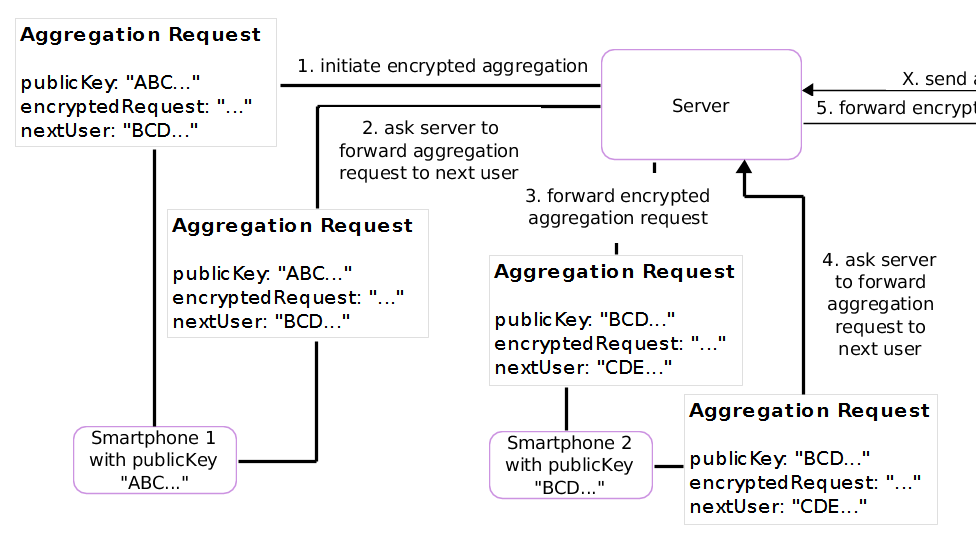
\includegraphics[width=\textwidth]{data/diagrams/decentral-encrypted-aggregation-4.png}
\end{figure}

 The aggregated results are available only to our research team in order to protect the research participants' privacy in case there is a privacy risk we have not thought of but the setting allows for them being available to the public. The aggregation requsts themselves are controlled by our research team and inserted on a daily basis.

 \subsection{Aggregation schemes}\label{aggregation-schemes}
 We found two types of aggregation requests to be of interest. First, the evalulation of mean values and second, the evaluation of more advanced statistical values such as median or other percentiles and distribution. The latter includes the possibility to calculate the former. Nevertheless, we want to test all research questions independently.
 We found the following aggregations to be especially of interest:
 \begin{enumerate}
 	\item Computing the average number of steps walked across all users participating in the request. (e.g. to calculate how many people reach the 10.000 steps per day\footnote{It has to be evaluated, which percentage of steps are registered because the phone will not always be on the person}.)
	\item Computing the average time spent walking, running, in a vehicle or on a bicycle\footnote{https://developers.google.com/android/reference/com/google/android/gms/location/DetectedActivity}.
	\item Computing how many people respectively which share of people combine using a bicycle with using a vehicle such as public transport or a car in one trajectory.
	\item How much time do people stay at work.
	\item How long do people travel to work.
	\item Where did many participants spend a significant amount of time on a certain day? (Event recognition)
	\item What percentage of whole travelling time do people spend on their bike, car, ...
	\item What is the average speed on roads.

	\item Collecting a list of the average number of steps walked by each participant during the timespan.
	\item Collecting a list of the duration of all registered activities.

	\item collecting a list of all trajectories registered by the users' phones.
 \end{enumerate}
 For all these and more aggregations, always both, the mean value and if possible, a complete list of values to compute other statistical figures are of interest.

 \subsection{Narrowing the area of the aggregation request}
 The aggregation requests outlined in the former subsection only provide useful data if the area of the aggregation can be limited e.g. to the scope of a city. Otherwise the resulting data would not allow for comparison and the scope of each aggregation would either be the whole user base which especially in the case of listing values would result in a huge amount of data passed around. Or, the limited number of participants in each aggregation would not be locally close which would 1. not result in useful data and 2. make it impossible to do aggregations as the average speed on roads. 
 In order to limit the area of aggregation and avoid sending the aggregation request to each user and leaving him with determining whether he is inside the area and participates in the request, the initiator of those requests has to now the location of users, respectively the location where the user is active the most.
 We do not see this as a violation of the user's privacy due to the following reasons:
 \begin{enumerate}
 	\item The exact location of the user e.g. the home or work location is not of interest at all. Rather the area for which the user can provide data is of interest. We propose to cluster location areas in a hierarchical structure similar to XXX and determine the granularity of the location published to the server as follows:
 	\begin{enumerate}
 		\item Each user sends the most coarse locational area as possible to the server - e.g. the continent.
 		\item If more than the required anonymity threshold of e.g. 10 active users are already registered with this location at the server, the server not only links this location to the user but also requests the user to send a less coarse location.
 		\item The user step by step sends a less coarse location e.g country, district, etc. until the server denies the location because not enough active users have registered with the location on this granularity level. It nevertheless increases the counter of users who requested access to this location. Once the counter exceeds a certain number, the server sends an aggregation request to participants in the more coarse area encompassing the requested less coarse area to determine the number of active users. If this number is above the required threshold, the granularity level for this location is made available and users can now register with this area and aggregation requests targeting this area can be send.
 		\item The fullfilment of the threshold has to be checked on a regular basis in order to close areas once the user base sinks below the anonymity threshold.
 	\end{enumerate}
 	In a more advanced setting, it should be possible to register with more than one area on the same level to avoid that a user e.g. living close to a city provides only data about the city or the bordering area. Nevertheless, 1. this should be limited to areas bordering each other to avoid user identification similar as in XX and 2. it has to be investigated whether this indeed not poses a risk or whether also the combination of areas needs to meet a certain anonymity threshold.
 \end{enumerate}

%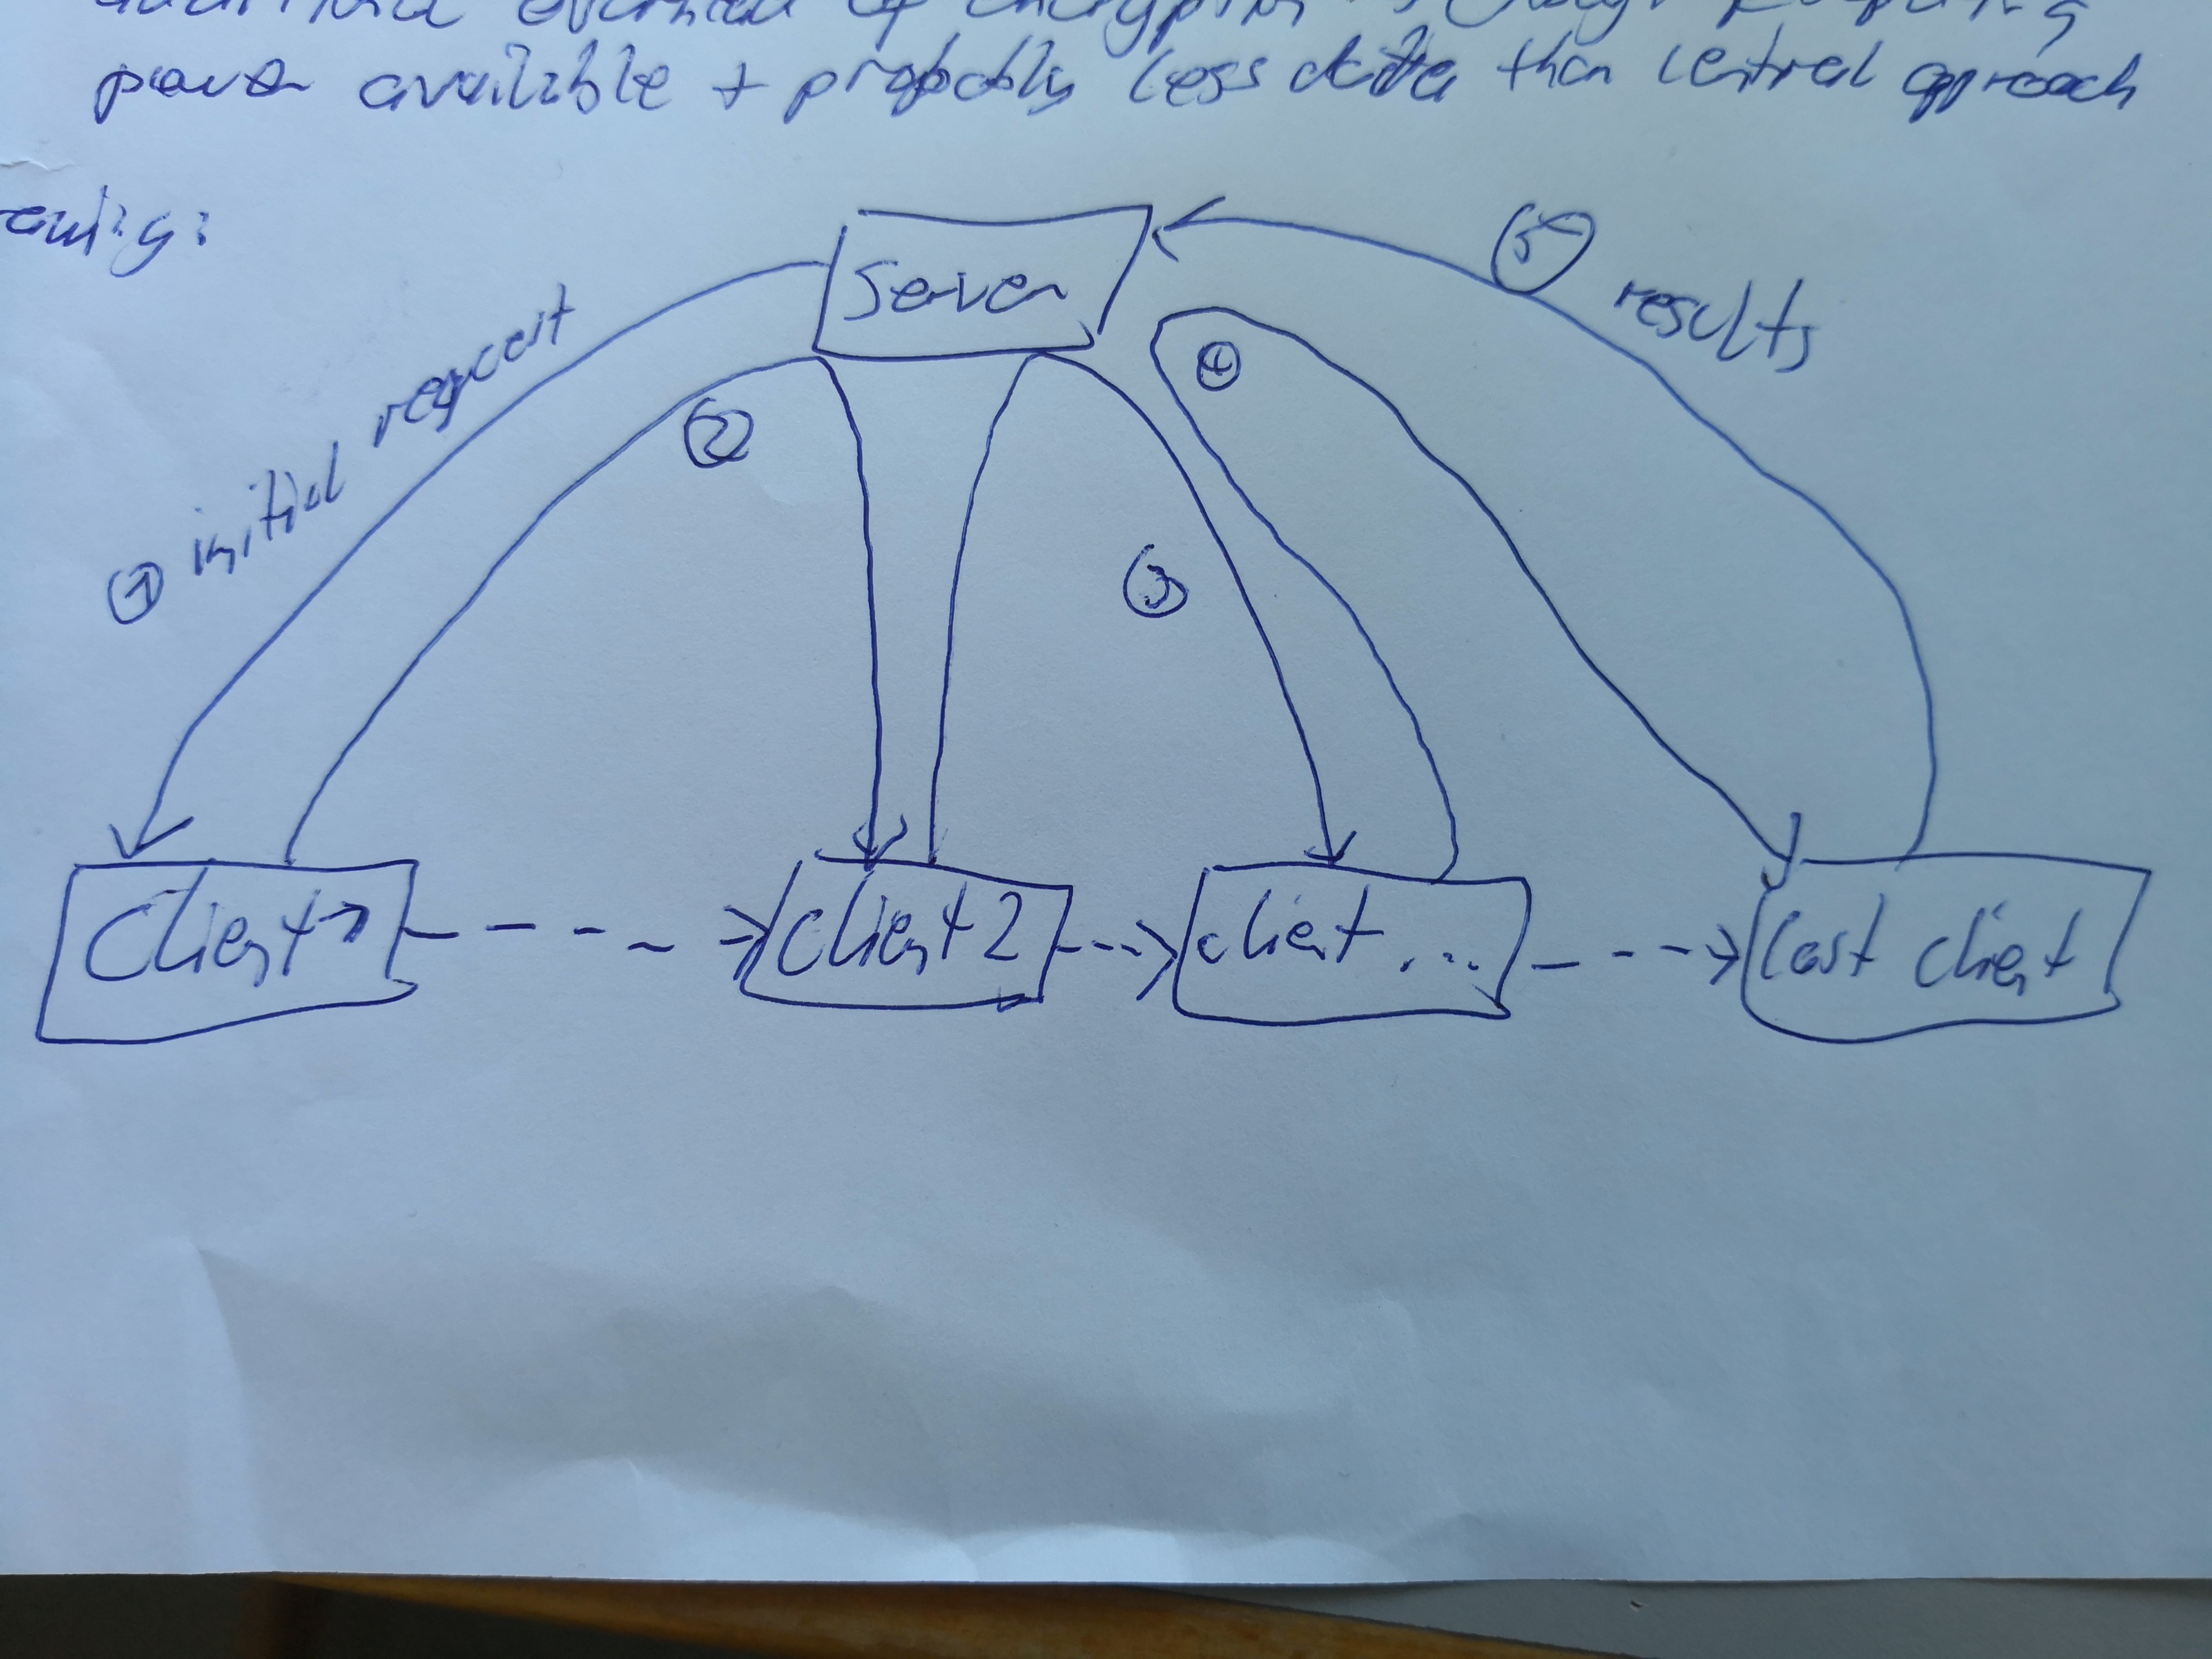
\includegraphics[width=\textwidth]{data/concept.jpg}